\chapter{GoogLeNet Model Architecture Details}\label{app:GoogLeNet}

In our GoogLeNet architecture, we use inception modules. In these modules, inputs go through four separate branches and are then concatenated together. For an inception layer denoted as Inception(A, B, C, D, E, F, G) the branches are defined as follows:

\begin{itemize}
    \item Branch 1: A simple $1 \times 1 \times 1$ convolution, taking A input channels to B output channels. This is followed by a batch normalization and a ReLU activation function.
    \item Branch 2: A $1 \times 1 \times 1$ convolution followed by a $3 \times 3 \times 3$ convolution. The first convolution takes A input channels to C output channels, followed by batch normalization and ReLU. This then goes to the next convolution layer, which outputs D channels using a kernel of size $3 \times 3 \times 3$. This is again followed by batch normalization and ReLU.
    \item Branch 3: A $1 \times 1 \times 1$ convolution followed by a $5 \times 5 \times 5$ convolution. The details are the same as for the other branches, but the first convolution takes A input channels to E output channels, and the next convolution outputs F channels.
    \item Branch 4: A max pool of kernel size $3 \times 3 \times 3$ is followed by a convolution of kernel size $1 \times 1 \times 1$ that takes A input channels to G output channels. This is followed once again by batch normalization and ReLU.
\end{itemize}

Here are full details for each layer of the GoogLeNet-based architecture:

\begin{itemize}
    \item Apply instance normalization to ECAL input.
    \item Convolution with 3D kernel of size 3, going from 1 input channel to 192 channels, with a padding of 1. This is followed by batch normalization and ReLU.
    \item Inception(192,  64,  96, 128, 16, 32, 32)
    \item Inception(256, 128, 128, 192, 32, 96, 64)
    \item Max pooling with a 3D kernel of size 3, a stride of 2, and padding of 1.
    \item Inception(480, 192,  96, 208, 16,  48,  64)
    \item Inception(512, 160, 112, 224, 24,  64,  64)
    \item Inception(512, 128, 128, 256, 24,  64,  64)
    \item Inception(512, 112, 144, 288, 32,  64,  64)
    \item Inception(528, 256, 160, 320, 32, 128, 128)
    \item Max pooling with a 3D kernel of size 3, a stride of 2, and padding of 1.
    \item Inception(832, 256, 160, 320, 32, 128, 128)
    \item Inception(832, 384, 192, 384, 48, 128, 128)
    \item Average pooling with a 3D kernel of size 7 and a stride of 1.
    \item The output array is flattened and concatenated with input $\phi$, $\eta$, total ECAL energy, and total HCAL energy.
    \item A densely connected layer with 1024 outputs, followed by ReLU.
    \item The output array is once again concatenated with the same input values.
    \item A final densely connected layer outputs 5 values, as in the architectures of the other two models.
\end{itemize}

The full architecture is shown in Figure~\ref{fig:gn_with_inceptin}.

\begin{figure}[htbp]
\centering
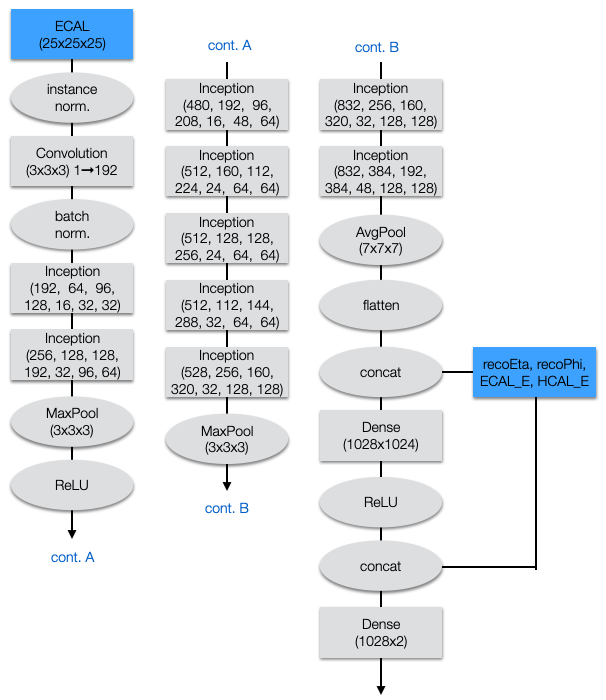
\includegraphics[width=0.38\textwidth]{Images/Calo/GN_architecture.png}
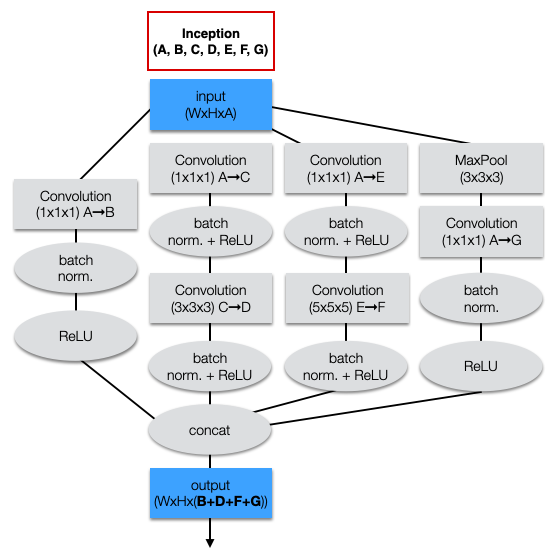
\includegraphics[width=0.38\textwidth]{Images/Calo/inception_architecture.png}
\caption{GoogLeNet-based architecture (top) and component inception architecture (bottom).
}
\label{fig:gn_with_inceptin}
\end{figure}